
\section{Plotting}


\subsection*{Basic Plotting Tools}

\begin{frame}[fragile]
  \frametitle{Basic \MTEX Plotting Tools}

General syntax:
\begin{lstlisting}
plot(object,<options>)
\end{lstlisting}

\begin{columns}
  \begin{column}{8.5cm}

    \only<1>{
      \lstset{emph={tight,jet,earea,smooth,antipodal},emphstyle={\color{blue}}}
    }

    \only<2|handout:0>{
      \lstset{emph={tight,jet,edist,smooth,antipodal},emphstyle={\color{blue}}}
    }

    \only<3|handout:0>{
      \lstset{emph={equal,earea,contourf,gray,antipodal},emphstyle={\color{blue}}}
    }


    Color range:

\begin{lstlisting}
tight, equal, [min max]
\end{lstlisting}

    Spherical projections:
\begin{lstlisting}
earea, edist, eangle, plain, 3d
\end{lstlisting}

    Filling:
\lstset{emph={scatter},emphstyle={}}
\begin{lstlisting}
scatter, smooth, contour, contourf
\end{lstlisting}

    Additional options:
\begin{lstlisting}
antipodal, complete, logarithmic
resolution, FontSize, grid, gray
\end{lstlisting}


  \end{column}

  \onslide<1->
  \begin{column}{3cm}
    \begin{overlayarea}{3cm}{6cm}
      \only<1|handout:0>{%
        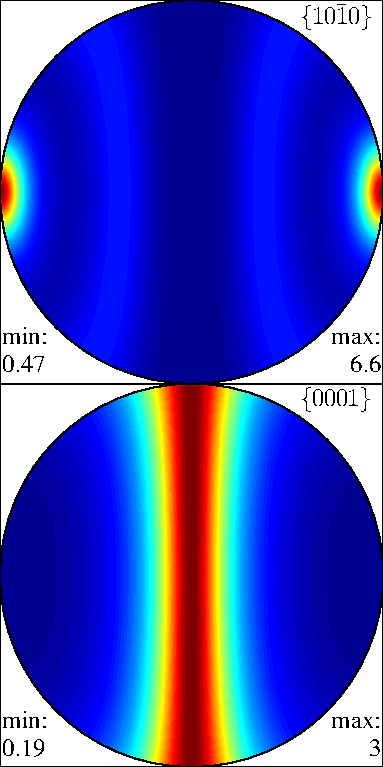
\includegraphics[width=3cm]{pic/fibreodf1}%
      }%
      \only<2>{%
        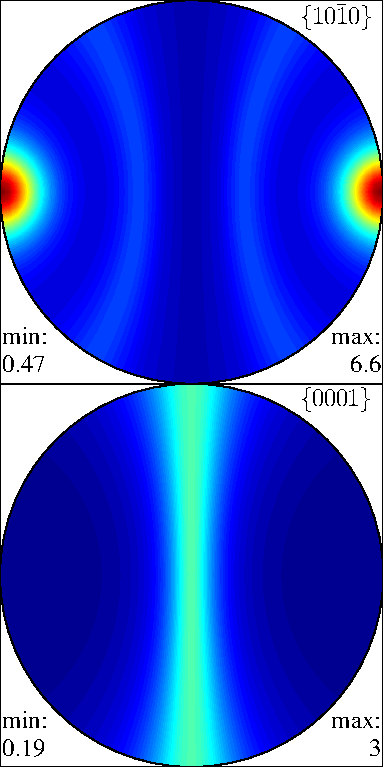
\includegraphics[width=3cm]{pic/fibreodf2}%
      }%
      \only<3|handout:0>{%
        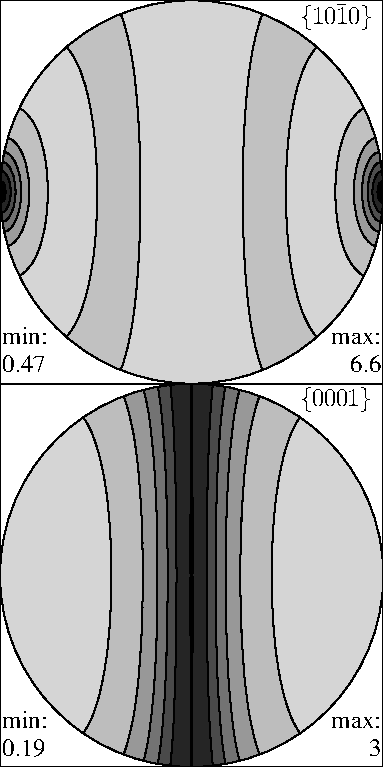
\includegraphics[width=3cm]{pic/fibreodf3}%
      }
    \end{overlayarea}
  \end{column}

\end{columns}


\end{frame}



\subsection*{Annotations}

\begin{frame}[fragile]
  \frametitle{Add Annotations to Pole Figure Plots}


\begin{columns}
  \begin{column}{8.5cm}

\begin{overprint}
  \onslide<1|handout:0>%
  General Syntax:%
\begin{lstlisting}
annotate(vector,<options>)
\end{lstlisting}
  \onslide<2|handout:1>%
  General Syntax:
\begin{lstlisting}
annotate(orientation,<options>)
\end{lstlisting}
\end{overprint}

Options:
\begin{lstlisting}
Marker            % marker shape
MarkerSize        % marker size
MarkerFaceColor   % face color
MarkerEdgeColor   % edge color
label             % a label text
color, background % text colors
\end{lstlisting}

\begin{overprint}
  \onslide<1|handout:0>%
  Example:
\begin{lstlisting}
annotate([xvector,yvector,zvector],
 'Backgroundcolor','w','Marker','s',
 'MarkerEdgeColor','w','labeled',
 'MarkerFaceColor','k')
\end{lstlisting}

  \onslide<2|handout:1>
Example:
\begin{lstlisting}
annotate(q0,'label','$q_0$',...
   'marker','s','MarkerSize',4,...
   'MarkerFaceColor','r','color','b')
\end{lstlisting}

\end{overprint}

\end{column}

  \begin{column}{3.5cm}
    \begin{overlayarea}{3.5cm}{7cm}
      \onslide<1->
      \only<1|handout:0>{%
        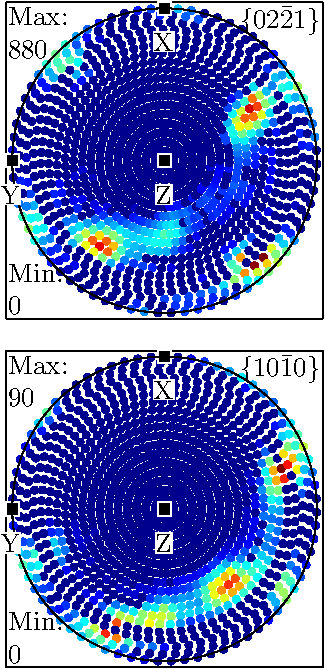
\includegraphics[width=3.5cm]{pic/annotationv}%
      }%
      \only<2>{%
        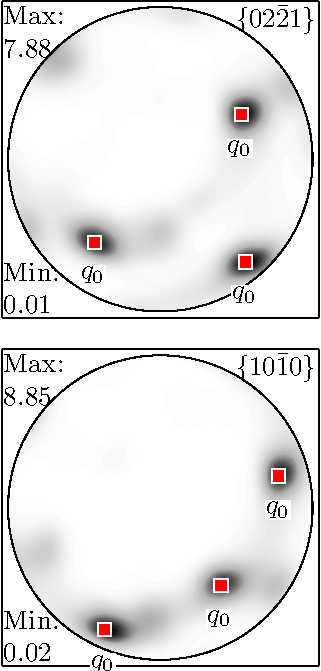
\includegraphics[width=3.5cm]{pic/annotationq}%
      }%
    \end{overlayarea}
  \end{column}

\end{columns}

\end{frame}

\subsection*{Annotations}

\begin{frame}[fragile]
  \frametitle{Add Annotations to ODF Plots}


\begin{lstlisting}
annotate(modalorientation(santafee),'Marker','s',...
  'MarkerSize',6,'MarkerFaceColor','red')
\end{lstlisting}

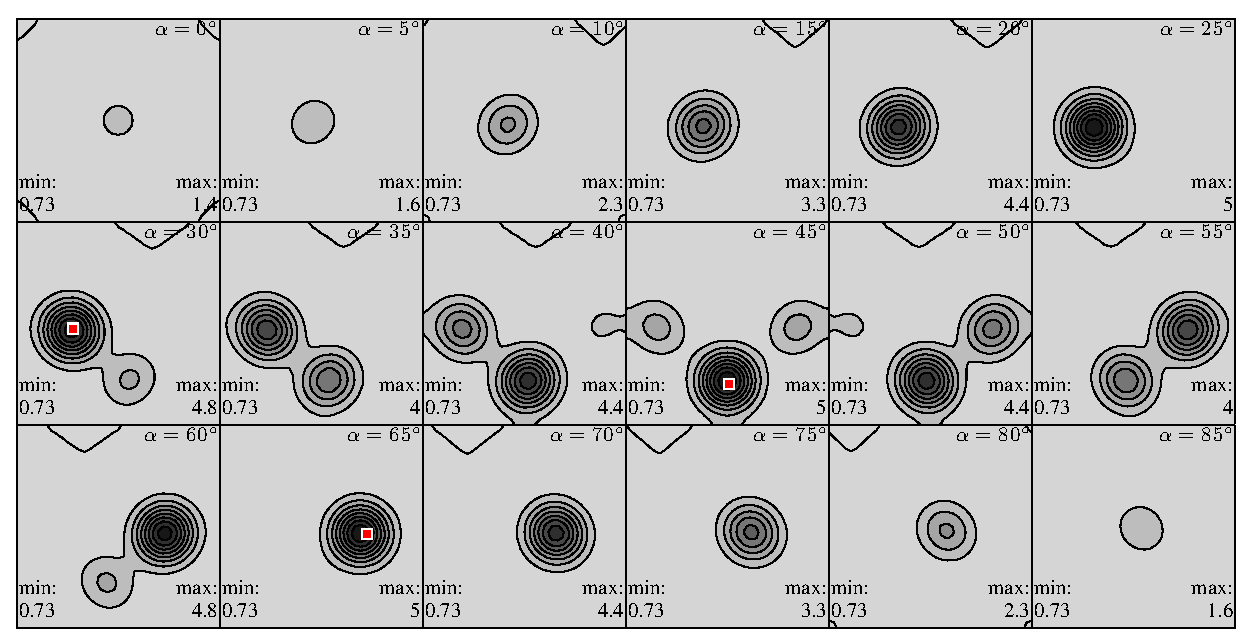
\includegraphics[width=\textwidth]{pic/odfanotate}

\end{frame}

\subsection*{Combined Plots}

\begin{frame}[fragile]
  \frametitle{Combining Different Data Into One Plot}

  \begin{columns}
    \begin{column}{8.7cm}

      General Syntax:%
\begin{lstlisting}
hold all; hold off
\end{lstlisting}

    Example:
\begin{lstlisting}
plotpdf(odf,h,'contourf','gray')

hold all

plotpdf(ebsd1,h,'MarkerEdgeColor','w',
 'MarkerColor','b','MarkerSize',5)

plotpdf(ebsd2,h,'MarkerEdgeColor','k',
 'MarkerColor','r','MarkerSize',5)

hold off
\end{lstlisting}


    \end{column}

    \begin{column}{3.5cm}
      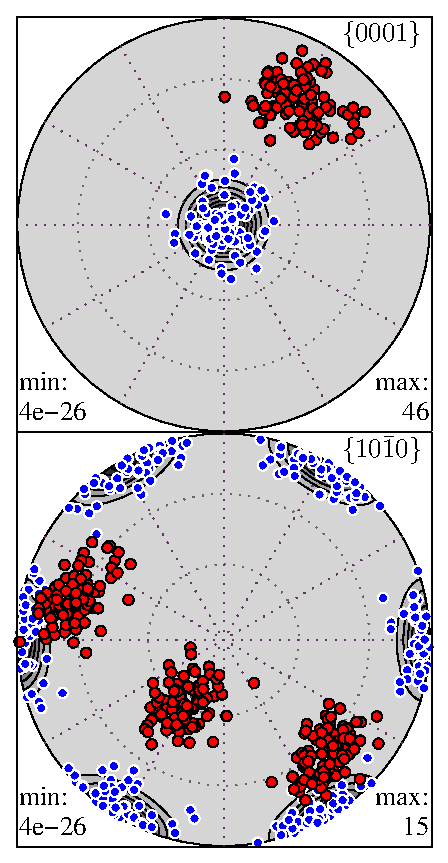
\includegraphics[width=3.5cm]{pic/combined}%
    \end{column}
  \end{columns}

\end{frame}

\subsection*{Export}

\begin{frame}[fragile]
  \frametitle{Exporting Graphics}
    Save a plot:
\begin{lstlisting}
savefigure(filename,<options>)
\end{lstlisting}

    \begin{block}{Formats}
      \begin{itemize}
      \item vector images: pdf, eps, ill
      \item bitmap images: jpg, tif, png, gif, bmp, pgm, ppm
      \end{itemize}

    \end{block}

    \begin{block}{Options}
\begin{lstlisting}
-append, -tiff, -cmyk, -adobecset
-r<resolution>
\end{lstlisting}
    \end{block}
\end{frame}


%%% Local Variables:
%%% mode: latex
%%% TeX-master: "main"
%%% End:
